\section{Analysis of vegetation density}
\label{sec:vegetation_analysis}
After the segmentation of the surface into different classes, the second objective of this thesis is to draw conclusions on vegetation density. Vegetation is one of the main factors to consider when looking for suitable emergency landing fields. Lower vegetation density increases the chances of a successful emergency landing.

One method for analyzing vegetation density with remotely sensed data are \emph{spectral vegetation indices} (SVIs). This chapter focuses on investigating several spectral vegetation indices and their usefulness with the data set presented in chapter~\ref{sec:dataset_analysis}.

\subsection{Spectral Vegetation Indices}
Spectral vegetation indices provide ways to indicate the vegetation density based on reflectances of visible and near-infrared (NIR) light spectrums. They rely on the fact that healthy vegetation absorbs most of the visible red and blue light while reflecting great portions of green light~\cite{glv03}.

Actually, the reflections of green light on plants is significantly higher than all other spectrums. This is what makes plants and vegetation appear green to the human eye. Other materials on earth's surface do not share this increased reflectance levels in the green spectrum. Building upon this knowledge, SVIs try to relate different spectral bands of light to predict vegetation density.

Most SVIs compare the difference between visible red light and NIR light~\cite{glv03}. The lower the amount of red light, the higher the density of green vegetation in the scene.

There are various indices that each combine the spectral bands in unique ways and perform slightly different color corrections. Most of the indices use simple algebraic formulas. In the end, they all produce a single scalar value indicating the density of the vegetation.

The next sections introduce some of the widely used vegetation indices.

\subsubsection{Ratio Vegetation Index}
The simplest SVI is the \emph{Ratio Vegetation Index} (RVI). It is represented by the ratio between NIR and red light~\cite{glv03} (see equation~\ref{eq:rvi}). Higher values indicate denser vegetation.

\begin{equation}
    \text{RVI} = \frac{\text{NIR}}{\text{Red}}
    \label{eq:rvi}
\end{equation}

Non-vegetated areas typically are below or near $1$. In that case the reflectance for NIR and red light are in the same order of magnitude. With increasing vegetation density, the amount of reflected red light shrinks, causing the index to grow. Extremely dense vegetation reaches a size of up to $30$.

The lower bound for the index is $0$, because negative values for the reflectances are not possible. On the other hand, there is no upper limit for the index. This makes it difficult to define from when exactly a vegetation is considered to be dense.

\subsubsection{Normalized Difference Vegetation Index}
One of the first approaches to monitor changes in global vegetation was driven by the National Oceanic and Atmospheric Administration (NOAA), a US agency focusing on the conditions of the environment. With the help of satellites and high-resolution radiometers they measured the earth's reflectance in five spectral bands, including red and NIR wavelengths. To support their analysis, they introduced a new vegetation index called the \emph{Normalized Difference Vegetation Index} (NDVI)~\cite{measuring_vegetation00}.

The NDVI was able to solve some of the shortcomings of the RVI. For example, because of the way it is calculated (see equation~\ref{eq:ndvi}), it is limited to the range of $-1$ to $1$. This makes it easier to categorize density levels for vegetation.

\begin{equation}
    \text{NDVI} = \frac{\text{NIR}-\text{Red}}{\text{NIR}+\text{Red}}
    \label{eq:ndvi}
\end{equation}

Values close to $1$ indicate a high probability for dense, green vegetation~\cite{gisg_ndvi20}. For lower values the density of the vegetation decreases. Values near $0$ do not allow for any precise conclusions about the surface conditions, except that living vegetation is very unlikely at that location. The negative range of values mostly consists of water.

\subsubsection{Enhanced Vegetation Index}
As time passes, improved measuring instruments were launched, like the Terra mission\footnote{see \url{https://terra.nasa.gov/}} of the National Aeronautics and Space Administration (NASA). The new instruments not only increased the resolution but also the precision of the spectral analysis. The more accurate data led to adjustments in the calculations for vegetation density, eventually resulting in the \emph{Enhanced Vegetation Index} (EVI)~\cite{modis2002}.

The EVI is calculated similarly to the NDVI, but has some additional factors to correct the influence of atmospheric conditions and background noise (see equation~\ref{eq:evi}). This means that EVI is more sensitive and offers more reliable information about the vegetation.

\begin{equation}
    \text{EVI} = G * \frac{
    \text{NIR}-\text{Red}
    }{
    \text{NIR} + C_1 * \text{Red} - C_2 * \text{Blue} + L
    }
    \label{eq:evi}
\end{equation}

$C_1$ and $C_2$ are coefficients to reduce the effects of aerosols. To filter out the distortions in the best possible way, also the spectral band of blue light is consulted for this. $L$ is a constant adjustment to address the issues of canopy background noise. Finally, $G$ is called the \emph{gain factor} and is used for linear scaling of the index. The values chosen in the original Terra mission are $C_1=6$, $C_2=7.5$, $L=1$ and $G=2.5$~\cite{modis2002}.

\subsubsection{Soil-Adjusted Vegetation Indices}
Another approach to improve the NDVI was made $1988$ by Alfredo Huete. He found NDVI to be unstable with factors like the soil color and moisture. Thus, he introduced the \emph{Soil-Adjusted Vegetation Index} (SAVI)~\cite{savi88} as another way to estimate vegetation density.

\begin{equation}
    \displaystyle
    \text{SAVI} =
    \bigg(
    \frac{\text{NIR} - \text{Red}}
    {\text{NIR} + \text{Red} + L}
    \bigg) * \big(1 + L \big)
    \label{eq:savi}
\end{equation}

As can be seen in equation~\ref{eq:savi}, Huete added a factor $L$ to correct unwanted influences of soil variations. In his experiments, he found $L=0.5$ to work best as a generic factor without further calibration~\cite{savi88}.

One issue with SAVI is, that proper soil adjustment also depends on vegetation density. Without any prior knowledge regarding vegetation it is difficult to find a value of $L$ that fits every situation. Qi et~al. presented another variation of SAVI, where they expressed $L$ with functional elements only~\cite{msavi94}. This version is called \emph{Modified Soil-Adjusted Vegetation Index} (MSAVI). It is listed in equation~\ref{eq:msavi}.

\begin{equation}
    \displaystyle
    \text{MSAVI} = \frac
    {
    2 \text{NIR} + 1
    - \sqrt{
    \big(2 \text{NIR}\big)^2
    - 8 \big(\text{NIR} - \text{Red}\big)
    }
    }
    {2}
    \label{eq:msavi}
\end{equation}

\subsection{Experiments}
To evaluate the usability of the SVIs this section focuses on applying them to some images picked from the data set. The images mostly consist of agricultural and forest areas. Special care was taken to ensure that the images contain many variations of vegetation. 

For the purpose of visualization, the output values of the indices are mapped to represent an 8-bit grayscale image. The brightness of the image indicates the density of the vegetation, with brighter patches implying denser vegetation. For the indices that do not have fixed limits, the ranges were selected in a way that resulted in a meaningful visualization. 

\newcommand{\VegetationIndicesImageWidth}{0.18\textwidth}
\begin{figure}
    \centering

    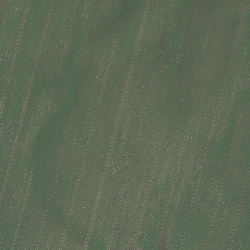
\includegraphics[width=\VegetationIndicesImageWidth]{images/vegetation/original/1} \hfill
    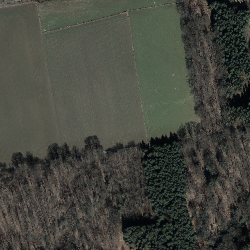
\includegraphics[width=\VegetationIndicesImageWidth]{images/vegetation/original/2} \hfill
    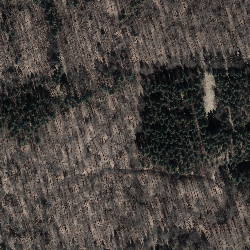
\includegraphics[width=\VegetationIndicesImageWidth]{images/vegetation/original/3} \hfill
    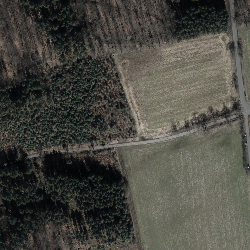
\includegraphics[width=\VegetationIndicesImageWidth]{images/vegetation/original/4} \hfill
    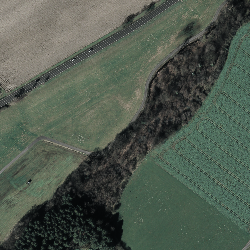
\includegraphics[width=\VegetationIndicesImageWidth]{images/vegetation/original/5}

    \vspace{3mm}
    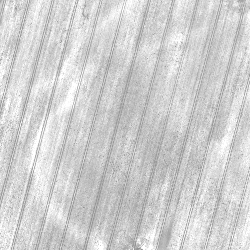
\includegraphics[width=\VegetationIndicesImageWidth]{images/vegetation/rvi/1} \hfill
    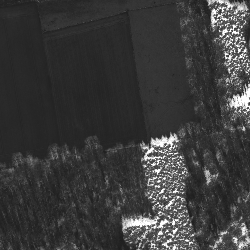
\includegraphics[width=\VegetationIndicesImageWidth]{images/vegetation/rvi/2} \hfill
    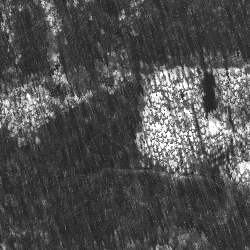
\includegraphics[width=\VegetationIndicesImageWidth]{images/vegetation/rvi/3} \hfill
    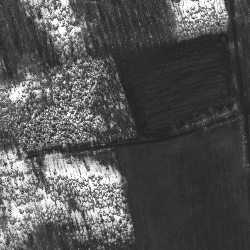
\includegraphics[width=\VegetationIndicesImageWidth]{images/vegetation/rvi/4} \hfill
    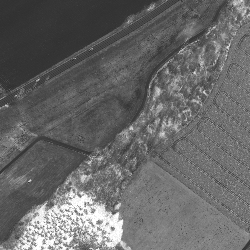
\includegraphics[width=\VegetationIndicesImageWidth]{images/vegetation/rvi/5}

    \caption{Vegetation analysis using RVI}
    \label{fig:vegetation_rvi_examples}
\end{figure}

Figure~\ref{fig:vegetation_rvi_examples} shows the vegetation density projection calculated with the RVI. Over the entire data set, RVI returned values in the range from $0$ to up to around $100$. Not taking outliers into account, most of the values were in range $0$ to $20$. This is also the range picked for the visualization. 

In the RVI the spots with most vegetation are green forests. Forests without foliage are clearly less vegetated according to the index (see middle column). For agricultural fields the separation is not so straightforward but still visible. For example, the fields in the last image shows only slightly different shades of gray. Interestingly, the fields in the leftmost image show up very bright compared to all other fields. 

In figure~\ref{fig:vegetation_ndvi_examples}, the projections of NDVI and EVI are presented. Both indices range from $-1$ to $1$, so the visualization also expresses that range. As can be seen, the projection for the two indices are quite different. 

\begin{figure}
    \centering

    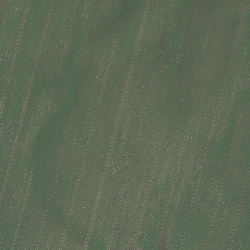
\includegraphics[width=\VegetationIndicesImageWidth]{images/vegetation/original/1} \hfill
    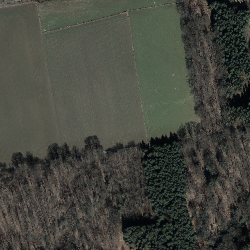
\includegraphics[width=\VegetationIndicesImageWidth]{images/vegetation/original/2} \hfill
    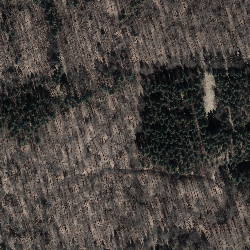
\includegraphics[width=\VegetationIndicesImageWidth]{images/vegetation/original/3} \hfill
    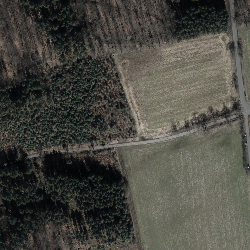
\includegraphics[width=\VegetationIndicesImageWidth]{images/vegetation/original/4} \hfill
    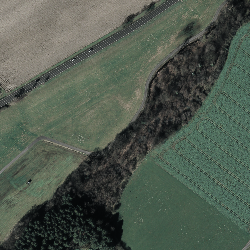
\includegraphics[width=\VegetationIndicesImageWidth]{images/vegetation/original/5}

    \vspace{3mm}
    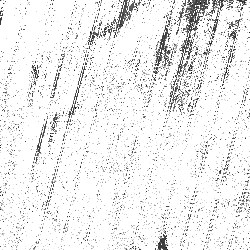
\includegraphics[width=\VegetationIndicesImageWidth]{images/vegetation/ndvi/1} \hfill
    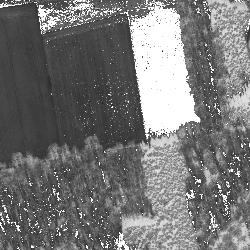
\includegraphics[width=\VegetationIndicesImageWidth]{images/vegetation/ndvi/2} \hfill
    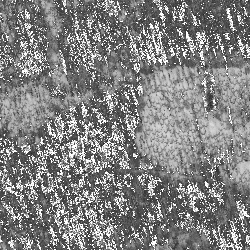
\includegraphics[width=\VegetationIndicesImageWidth]{images/vegetation/ndvi/3} \hfill
    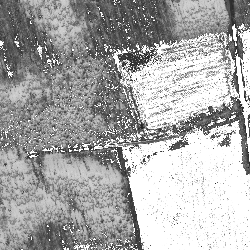
\includegraphics[width=\VegetationIndicesImageWidth]{images/vegetation/ndvi/4} \hfill
    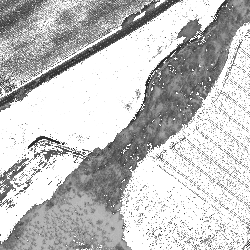
\includegraphics[width=\VegetationIndicesImageWidth]{images/vegetation/ndvi/5}

    \vspace{3mm}
    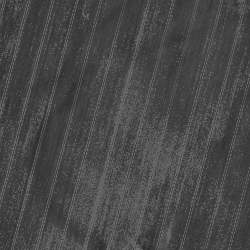
\includegraphics[width=\VegetationIndicesImageWidth]{images/vegetation/evi/1} \hfill
    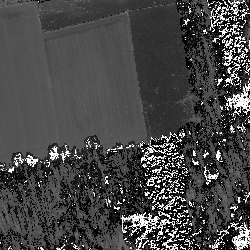
\includegraphics[width=\VegetationIndicesImageWidth]{images/vegetation/evi/2} \hfill
    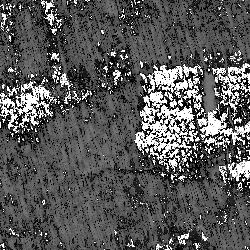
\includegraphics[width=\VegetationIndicesImageWidth]{images/vegetation/evi/3} \hfill
    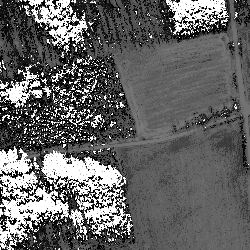
\includegraphics[width=\VegetationIndicesImageWidth]{images/vegetation/evi/4} \hfill
    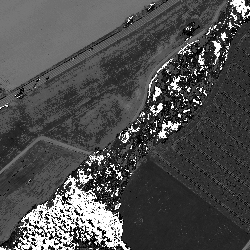
\includegraphics[width=\VegetationIndicesImageWidth]{images/vegetation/evi/5}

    \caption{Vegetation analysis using NDVI and EVI}
    \label{fig:vegetation_ndvi_examples}
\end{figure}

For example, the leftmost image is very bright for NDVI but rather dark for EVI. In fact, EVI's results are almost the exact opposite of NDVI for this image. While the lane tracks in this image are dark for NDVI, they are actually brighter in the EVI. These conflicting results for agricultural fields are also visible in the other images. 

Although the results contradict each other, when viewed for each index separately the result could be plausible. Both NDVI and EVI indicate different levels of vegetation for agricultural fields, even if the colored images only show minor differences. Particularly in the second and fifth image this becomes evident.

With regards to forests, NDVI performs rather bad. The middle image shows that there is almost no difference in the projection, regardless of the foliage. In contrast, EVI is able to make a clear distinction. For trees with foliage there are large bright spots in the projections.

Lastly, figure~\ref{fig:vegetation_savi_examples} presents the visualizations for SAVI and MSAVI. For SAVI the ranges from $0$ to $20$ and for MSAVI from $0$ to $80$ are visualized. In general, the projections of MSAVI yielded much higher values than SAVI. That is why the visualizations of MSAVI are much brighter. 

\begin{figure}
    \centering

    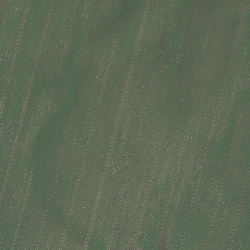
\includegraphics[width=\VegetationIndicesImageWidth]{images/vegetation/original/1} \hfill
    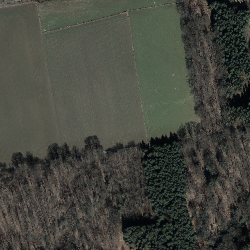
\includegraphics[width=\VegetationIndicesImageWidth]{images/vegetation/original/2} \hfill
    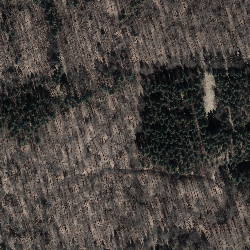
\includegraphics[width=\VegetationIndicesImageWidth]{images/vegetation/original/3} \hfill
    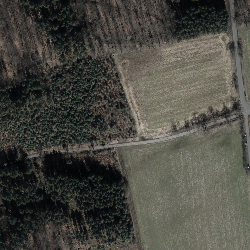
\includegraphics[width=\VegetationIndicesImageWidth]{images/vegetation/original/4} \hfill
    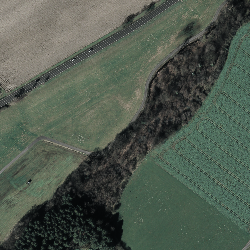
\includegraphics[width=\VegetationIndicesImageWidth]{images/vegetation/original/5}

    \vspace{3mm}
    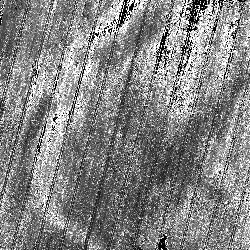
\includegraphics[width=\VegetationIndicesImageWidth]{images/vegetation/savi/1} \hfill
    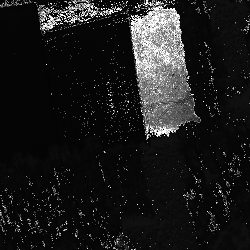
\includegraphics[width=\VegetationIndicesImageWidth]{images/vegetation/savi/2} \hfill
    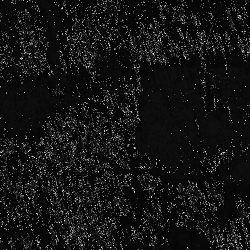
\includegraphics[width=\VegetationIndicesImageWidth]{images/vegetation/savi/3} \hfill
    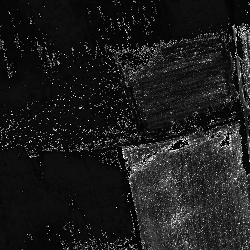
\includegraphics[width=\VegetationIndicesImageWidth]{images/vegetation/savi/4} \hfill
    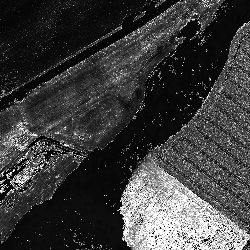
\includegraphics[width=\VegetationIndicesImageWidth]{images/vegetation/savi/5}

    \vspace{3mm}
    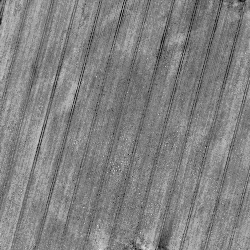
\includegraphics[width=\VegetationIndicesImageWidth]{images/vegetation/msavi/1} \hfill
    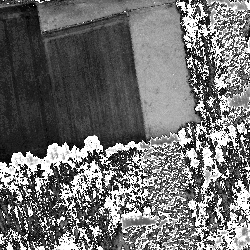
\includegraphics[width=\VegetationIndicesImageWidth]{images/vegetation/msavi/2} \hfill
    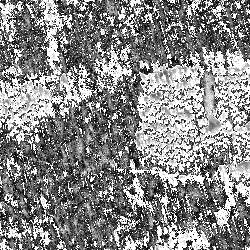
\includegraphics[width=\VegetationIndicesImageWidth]{images/vegetation/msavi/3} \hfill
    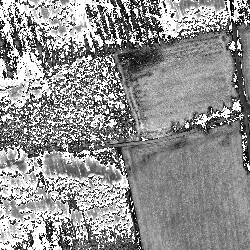
\includegraphics[width=\VegetationIndicesImageWidth]{images/vegetation/msavi/4} \hfill
    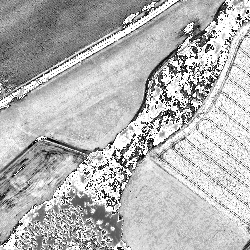
\includegraphics[width=\VegetationIndicesImageWidth]{images/vegetation/msavi/5}

    \caption{Vegetation analysis using SAVI and MSAVI}
    \label{fig:vegetation_savi_examples}
\end{figure}

Both SAVI and MSAVI do not tell a big difference about forest areas. Regardless of any foliage, the indices always show similar projections.

For agriculture however, both indices are very opinionated. Even in spots where the original images hardly show any differences, SAVI and MSAVI project a considerable contrast in vegetation density. Again, the second and fifth image show this very clearly.

\subsection{Discussion}
\WIP{
assumption: forest does not necessarily have more vegetation. depends on type of trees and heavilty on foliage. also type of crops make big difference. 

chosen images include living and dead vegetation to see if indices can tell the difference. best case is very distinct values for living/dead vegetation.

actual vegetation can only be estimated based on visual aspects of dataset. Dataset doesn't tell anything about real situation of vegetation for the areas. So it is hard to tell if results from SVIs are accurate.

data set consists of RGB and NIR light values. most SVIs are created for specific set of hardware. mostly deployed on satellites, so SVIs take into account atmospheric effects on data. however, images in our data set are taken from airplanes with different cameras. so data set might not be applicable for the SVIs. \footnote{\url{https://www.opengeodata.nrw.de/produkte/geobasis/lbi/dop/dop_jp2_f10/}}
% TODO: which hardware used for data? how collected?

predicions of different SVIs are not consistent. spots with dense vegetation vary depending on the SVI used. which one is right? hard to tell without seeing the actual vegetation situation.

conclusion: use SVIs with care, because results vary a lot. with more information about image data, better assessment for projections can be made. maybe also play with factors in SVIs to adjust for implications of very specific hardware.

\newpage
